\documentclass{article}

\usepackage{makecell, graphicx}
\graphicspath{ {./images/} }

\title{Ch. 15 CW \#1 Solutions}
\author{Principles of Microeconomics}
\date{\today}

\begin{document}

\maketitle

\section*{15.1. What is a Competitive Market}

\begin{enumerate}

\item 

	\begin{enumerate}
	
	\item No, there aren't many sellers.
	
	\item Yes, natural gas is exactly the same regardless of the producer; there are many buyers of natural gas, and the problem makes it sound like there are many sellers.
	
	\item No, the products aren't all the same.
	
	\item No, each market has at most one or two ticket sellers, so there aren't many sellers.
	
	\end{enumerate}
	
\item (c) -- In a perfectly competitive market, firms are price takers.

\item

	\begin{enumerate}
	
	\item Milk is essentially the same regardless of the producer, and there are many buyers and sellers.
	
	\item
	
		\begin{center}
		\begin{tabular}{c | c | c | c | c }
		Quantity & Price & \makecell{Total\\Revenue} & \makecell{Average\\Revenue} & \makecell{Marginal\\Revenue} \\
		\hline
		1 gallon & \$6 & \$6 & \$6 & \$6 \\
		\hline
		2 & 6 & 12 & 6 & 6 \\
		\hline
		3 & 6 & 18 & 6 & 6 \\
		\hline
		4 & 6 & 24 & 6 & 6 \\
		\hline
		5 & 6 & 30 & 6 & 6 \\
		\hline
		6 & 6 & 36 & 6 & 6 \\
		\hline
		7 & 6 & 42 & 6 & 6 \\
		\hline
		8 & 6 & 48 & 6 & 6
		\end{tabular}
		\end{center}
	
	\end{enumerate}
	
\item (c) -- Marginal revenue is the price of the good which is constant in a perfectly competitive industry. Total revenue is $PQ$, so it's proportional to the quantity sold. If quantity increases by 10\%, total revenue increases by 10\%.

\section*{15.2. The Competitive Firm's Supply Curve}

\item

	\begin{enumerate}

	\item Marginal benefit is the number of deaths due to disease that inoculation prevents. Marginal cost is the number of deaths that inoculation causes. 
	
		\begin{center}
		\begin{tabular}{c | c | c }
		MB & MC & Profit \\
		\hline
		10 & 0 & 10 \\
		9 & 1 & 18 \\
		8 & 2 & 24 \\
		7 & 3 & 28 \\
		6 & 4 & 30 \\
		5 & 5 & 30 \\
		4 & 5 & 29 \\
		3 & 5 & 27 \\
		2 & 5 & 24 \\
		1 & 5 & 20
		\end{tabular}
		\end{center}
		
	\item Between 50\% and 60\% of the population should be inoculated because that saves the highest number of people, 30. Note that it's where $MC = MB$.
	
	\item Profit is the net number of loves saved -- the deaths due to disease prevented minus the deaths due to inoculation. See part (a) for the calculation.
		
	\end{enumerate}
	
\item In the summer, lobster is locally available and cheaper. For the rest of the year, the shacks have to source lobster from around the world which is more expensive. Sourcing the lobster from around the world increases the shacks' variable costs. They shut down when their average variable costs are higher than the price that they can receive for their lobster. That's optimal because they save more money (their variable cost) than they give up (their revenue). 

\item

	\begin{enumerate}
	
	\item $MC$
	
	\item $AVC$
	
	\item $AVC$; $ATC$
	
	\item $ATC$
	
	\end{enumerate}

\newpage
	
\item \phantom{x}

	\begin{center}
	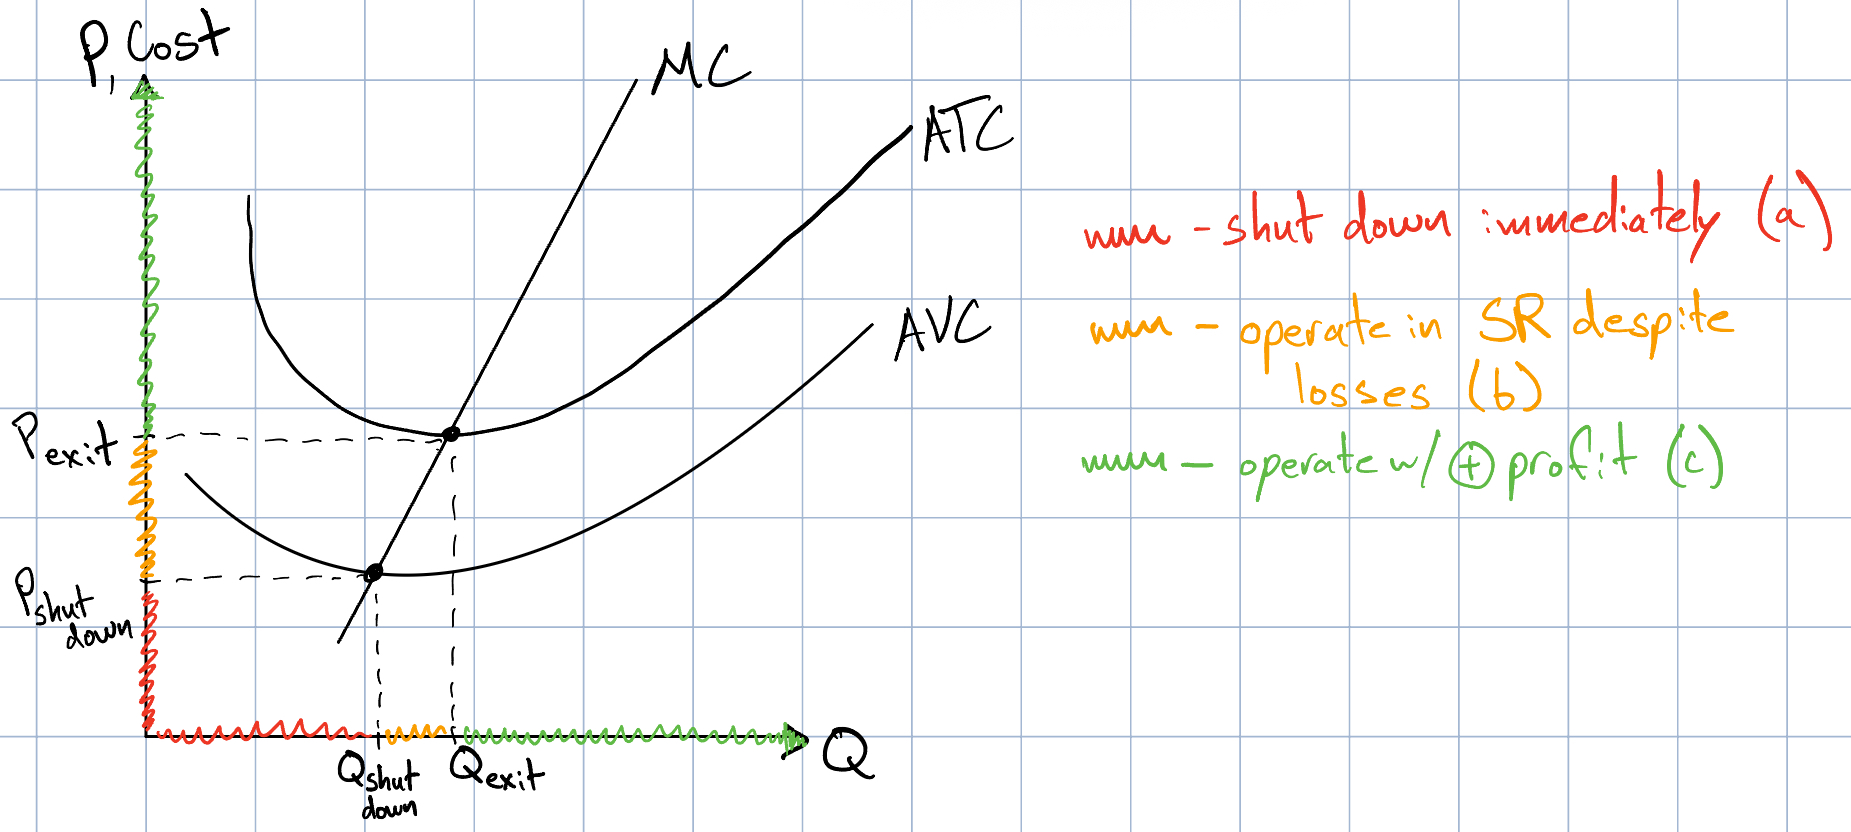
\includegraphics[width = \textwidth]{q8}
	\end{center}
	
\item \phantom{x}

	\begin{center}
	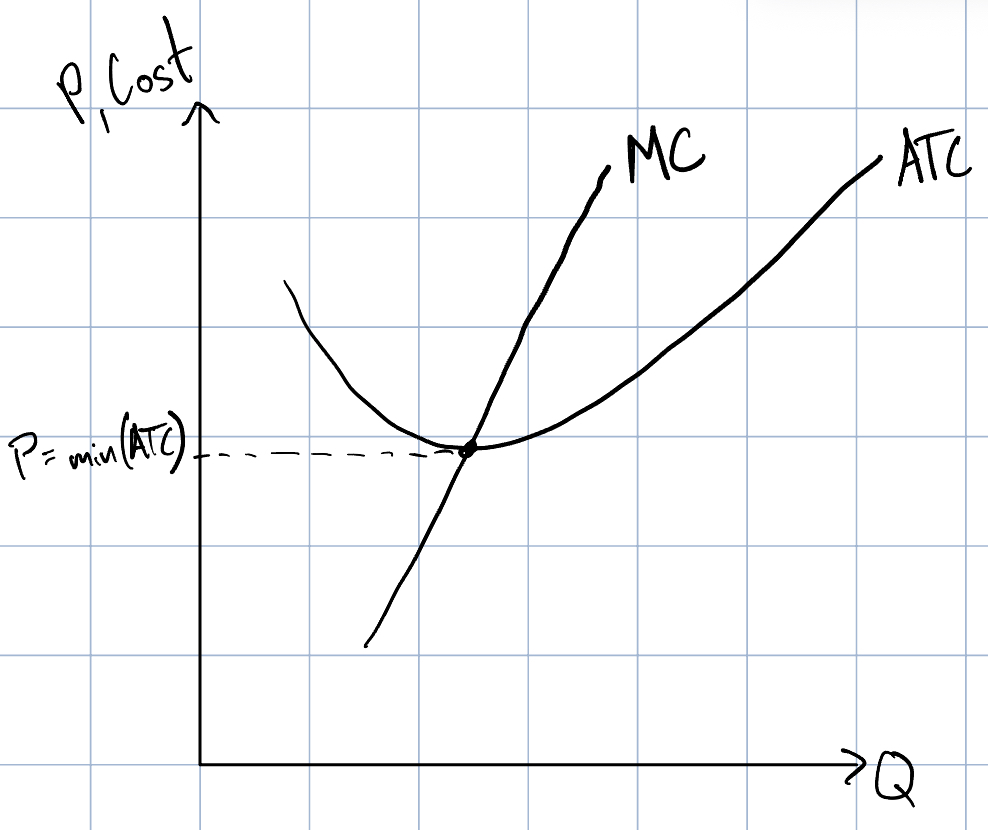
\includegraphics[width = 0.5\textwidth]{q9}
	\end{center}

\end{enumerate}

\end{document}